% @author {Arlet Acosta González}
% @email {arletacostagonzalez@gmail.com}
% @year 2023
% @version 1.0
% @license CC BY 4.0
%
% Se agradecen sus comentarios, contribuciones, reporte de bugs y la difusión de esta plantilla.




% Tipo de documento ytamaño de letra
\documentclass[10pt]{article}

% Ajuste de lenguaje
\usepackage[spanish, english]{babel}

% Tamaño de página y margenes
\usepackage[letterpaper, top=2.5cm,bottom=3.5cm, left=3cm, right=2.5cm, marginparwidth=1.75cm]{geometry}

% Permite manejo de ecuaciones y símbolos matemáticos
\usepackage{amsmath, amssymb, amsthm, amsfonts}

% Paquete para agregar imágenes
\usepackage{graphicx}

% Paquete para hipervinculos
\usepackage{hyperref}
\hypersetup{
    colorlinks=true,
    linkcolor=black,
    urlcolor=black,
    citecolor=black}

% Package for specifying fonts
\usepackage{fontspec}

% Permite el manejo de caracteres especiales en el español
\usepackage[utf8]{inputenc} 
\usepackage[T1]{fontenc}

% Subrayado de textos
\usepackage[normalem]{ulem}

% Personalizar los encabezados y pies de página
\usepackage{fancyhdr}
\pagestyle{fancy}

\usepackage{tabularx}
% Ruta para imagenes
\graphicspath{{image/}}

% Fuente principal del texto: Arial
\setmainfont{Arial}

% Ajusta la sangría
\setlength{\parindent}{1cm}

% Ajusta el espacio entre renglones
\setlength{\parskip}{0.5cm}

% Headers config
% Cambiar Volumen, Numero y páginas
\lhead{Inteligencia Artificial en la Medicina. \\Aplicaciones y dilemas éticos}
\rhead{
    
\includegraphics[width=4cm]{logo_usal_footer2.png}}
\headsep=60pt

% Referencias
\usepackage[
backend=biber,
style=numeric,
sorting=none
]{biblatex}
\addbibresource{Ref MI.bib}




% Información del artículo

\title{\Huge La Inteligencia Artificial en la Medicina. Principales aplicaciones y dilemas éticos}
\author{\Large Arlet Acosta González}

\date{\normalsize Universidad de Salamanca\\
\textit{arlet.acosta@usal.es}}


\begin{document}
\begin{figure}
    \centering
    
\includegraphics[width=0.5\linewidth]{logo_usal_footer2.png}
     \label{fig:enter-label}
\end{figure}

\maketitle


\selectlanguage{spanish}
\begin{abstract}
    \textit{\normalsize El presente artículo constituye una revisión de la presencia de la Inteligencia Artificial (IA) en la Medicina. Primeramente, se introduce el concepto de Inteligencia Artificial definido por John McCarthy en 1956.  Se revisa exhaustivamente la presencia y las aplicaciones de la IA en la Medicina, desde su definición inicial por John McCarthy en 1956 hasta su integración actual en diversas áreas de la atención sanitaria. Además, se exploran los dilemas éticos que surgen al emplear estas tecnologías avanzadas en la toma de decisiones médicas y el manejo de datos sensibles.Se comentan algunos ejemplos concretos del empleo de la IA en las diferentes áreas de aplicación sanitaria, así como en diferentes especialidades médicas. Finalmente se analizan las implicaciones éticas de del uso de estas tecnologías en la Medicina.}
    
    \vspace{0.5cm}

    \textbf{Palabras clave:} Inteligencia Artificial (IA), aplicaciones, Medicina, ética.
\end{abstract}


\selectlanguage{english}
\begin{abstract}
    \textit{\normalsize This article constitutes a review of the presence of Artificial Intelligence (AI) in Medicine. First, the concept of Artificial Intelligence defined by John McCarthy in 1956 is introduced. The presence and applications of AI in Medicine are exhaustively reviewed, from its initial definition by John McCarthy in 1956 to its current integration in various areas of care. . sanitary. Additionally, the ethical dilemmas that arise when using these advanced technologies in medical decision-making and the handling of sensitive data are explored. Some specific examples of the use of AI in different areas of healthcare application, as well as in different specialties, are discussed. medical. Finally, the ethical implications of the use of these technologies in Medicine are analyzed.}
    
    \vspace{0.5cm}

    \textbf{Keywords:} Artificial Intelligence (AI), applications, Medicine, ethic.
\end{abstract}

\selectlanguage{spanish}
\begin{center}
    \section{Introducción}
\end{center}

La rápida evolución de la Inteligencia Artificial (IA) ha transformado diversos campos, y su influencia en el ámbito médico se ha vuelto cada vez más prominente.
Desde la Conferencia de Dartmouth en 1956, la IA ha sido conceptualizada como la ciencia y la ingeniería dedicada a crear máquinas inteligentes capaces de imitar funciones cognitivas humanas. Este conjunto de Tecnologías de Información y Comunicaciones (TIC) avanzadas abarca desde la percepción hasta el aprendizaje, el razonamiento y la resolución de problemas, desempeñando un papel crucial en la mejora de la eficiencia y la eficacia en la prestación de servicios de salud.

En la última década, la investigación en IA aplicada a la medicina ha experimentado un crecimiento significativo. La capacidad de los algoritmos de IA para analizar grandes cantidades de datos ha revolucionado la prevención, diagnóstico y tratamiento de diversas enfermedades. La IA ha permeado diversas áreas de la medicina, desde la prevención de enfermedades y diagnóstico precoz hasta el tratamiento y seguimiento de pacientes. Algoritmos informáticos especializados contribuyen a la identificación temprana de enfermedades como el cáncer y la detección de patrones en imágenes médicas, optimizando el proceso de diagnóstico y permitiendo tratamientos más personalizados. La integración de datos provenientes de exámenes médicos, registros electrónicos y aplicaciones para dispositivos móviles permite una toma de decisiones clínicas más precisa y eficiente.
Sin embargo, este avance no está exento de dilemas éticos. La gestión de datos médicos sensibles plantea cuestionamientos sobre la privacidad y la posibilidad de discriminación. ¿Cómo se garantiza que la información genética no se utilice con fines perjudiciales? Estas interrogantes son esenciales en un contexto donde la IA busca mejorar la atención médica de manera ética y responsable.
El avance de la IA en la medicina plantea desafíos éticos fundamentales. La seguridad de los sistemas, la transparencia en la toma de decisiones y la responsabilidad de los diseñadores y constructores son aspectos críticos. La Unión Europea ha establecido principios que subrayan la importancia de centrar la IA en el ser humano, garantizar valores éticos y abogar por la privacidad y la equidad.



\newpage % Agrega o elimina estos saltos de página de acuerdo a tus necesidades.
\vspace{0.5cm}
\begin{center}
    \section{Objetivos}
\end{center}
\begin{itemize}
  \item Analizar la evolución de la Inteligencia Artificial (IA) hasta su integración actual en diversas áreas de la Medicina.
  \item Revisar y discutir ejemplos específicos de aplicaciones de la IA en diferentes campos de la atención sanitaria y especialidades médicas.
  \item Examinar las implicaciones éticas asociadas al uso de la IA en la Medicina, centrándose en cuestiones de privacidad, discriminación y responsabilidad.
  \item Evaluar los desafíos éticos fundamentales relacionados con la seguridad de los sistemas, la transparencia en la toma de decisiones y la responsabilidad de los diseñadores y constructores de tecnologías de IA en el ámbito médico.
  \end{itemize}

 
\vspace{0.5cm}
\begin{center}
    \section{Metodología}
\end{center}


Se llevó a cabo una revisión exhaustiva de la literatura científica relacionada con la presencia de la Inteligencia Artificial en la Medicina. 


Se recopilaron y analizaron estudios, artículos y documentos relevantes desde la Conferencia de Dartmouth en 1956 hasta la actualidad. 


Revisión y síntesis de conceptos clave, ejemplos específicos de aplicaciones en diversas áreas médicas, así como el análisis de las implicaciones éticas asociadas al uso de la IA en el ámbito sanitario. Se hizo especial hincapié en la normativa ética propuesta por la Unión Europea y los Principios de la IA de Asilomar en EE. UU. 


La conclusión final se formuló considerando los hallazgos obtenidos durante la revisión bibliográfica y el análisis crítico de la información recopilada.

\vspace{0.5cm}
\begin{center}
    \section{¿Qué es la Inteligencia Artificial (IA)?}
\end{center}

La Conferencia de Darmouth de 1956 es considerada como la ocasión en que se define por John McCarthy, el término de Inteligencia Artificial (IA, por sus siglas en inglés): “Es la ciencia y la ingeniería de fabricar máquinas inteligentes, especialmente programas informáticos inteligentes. Está relacionado con la tarea similar de usar computadoras para comprender la inteligencia humana, pero la IA no tiene que limitarse a métodos que sean biológicamente observables.”\cite{mccarthy_what_nodate}


Si bien no existe una definición única de IA, en general, es conceptualizada como un conjunto de Tecnologías de Información y Comunicaciones (TIC) avanzadas, consistentes en “máquinas capaces de imitar ciertas funcionalidades de la inteligencia humana, incluidas características tales como percepción, aprendizaje, razonamiento, resolución de problemas, interactuación con el lenguaje e incluso producción de trabajos creativos”.


La enunciación ha sido propuesta por la Comisión Mundial de Ética del Conocimiento Científico y la Tecnología de la UNESCO (COMEST, según sus siglas en inglés). Se trata de un conjunto de tecnologías a través de las cuales las máquinas inteligentes están adquiriendo la capacidad de aprender, mejorar y tomar decisiones calculadas de manera que les permiten realizar tareas que antes se pensaba que se basaban únicamente en la experiencia, la creatividad y el ingenio humanos. La IA consiste en general en una gama de capacidades cognitivas “similares a las humanas” realizadas por máquinas. Puede estar basado en software y/o integrado en hardware específico. \cite{drnas_de_clement_inteligencia_2022}
\vspace{0.5cm}
\begin{center}
    \section{Inteligencia Artificial en Medicina}
\end{center}


Durante la última década, la investigación de IA aplicada en medicina ha crecido a pasos agigantados. De hecho, solo en 2016 hubo mucha más inversión en iniciativas de IA en medicina que en otras áreas de la economía mundial. ¿Qué factores explican este mayor interés? Una de las posibles razones es la gran capacidad de la IA para mejorar la eficiencia y eficacia de la prestación de servicios de salud.


Entonces, ¿qué pueden hacer los algoritmos de IA por el futuro de la medicina? Es un hecho ineludible que, en el mundo desarrollado, la cantidad de datos relacionados a la salud de cada persona aumenta constantemente, y que la calidad y consolidación de estos en muchos países aún es dudosa. Sin embargo, se está avanzando en la dirección correcta para mejorarlos, principalmente a través de la digitalización de los sistemas informáticos relacionados con los registros médicos electrónicos, la interoperabilidad y protocolos de comunicación seguros que garantizan que el acceso, tratamiento y uso de los datos se lleven a cabo en conformidad con la ley. En este sentido, solo cabe una pregunta: ¿qué hacemos con los datos médicos? Aquí es donde la IA juega un papel central. Con la cantidad de exámenes que se hacen los pacientes, una decodificación del DNA menos costosa y los datos que proporcionan los mismos sujetos a través de aplicaciones para Smartphones u otros dispositivos, se requieren mecanismos avanzados en el procesamiento de estos y el reconocimiento de patrones para la toma de decisiones clínicas relevantes. La figura 1 muestra la integración de varias fuentes de datos relacionadas con los pacientes y el procesamiento respectivo, mediante técnicas de inteligencia artificial.

Entre todos los datos también encontramos aquellos provenientes de las redes sociales y los proporcionados por las personas a través de aplicaciones de teléfonos inteligentes relacionados con la atención médica. El resultado final apunta a que múltiples usuarios, empezando por el paciente, puedan hacer un uso correcto de este nuevo conocimiento, el cual es clave en la asistencia sanitaria.


No cabe duda de que la IA está provocando una gran revolución positiva en cuanto a la salud de las personas. Sin embargo, no todo es color de rosas. Al tratarse de datos personales sensibles, su tratamiento debe realizarse bajo estrictas medidas de seguridad y consideraciones éticas. Efectivamente, ¿qué pasaría si analizando los datos del DNA de un individuo, se detecta que tiene una alta probabilidad de desarrollar diabetes en el futuro? ¿Cubrirá el seguro de salud esta enfermedad? ¿Sufrirá algún tipo de discriminación? No debemos olvidar que el foco de la IA en salud es ayudar a las personas de forma ética y responsable, cuidando que sus datos personales no se utilicen para fines distintos a los de potenciar su bienestar o curar enfermedades que les puedan afectar. De ninguna manera pueden ser utilizados para otros fines que violen los derechos humanos fundamentales.\cite{ruiz_inteligencia_2023} 


\begin{figure}
    \centering
    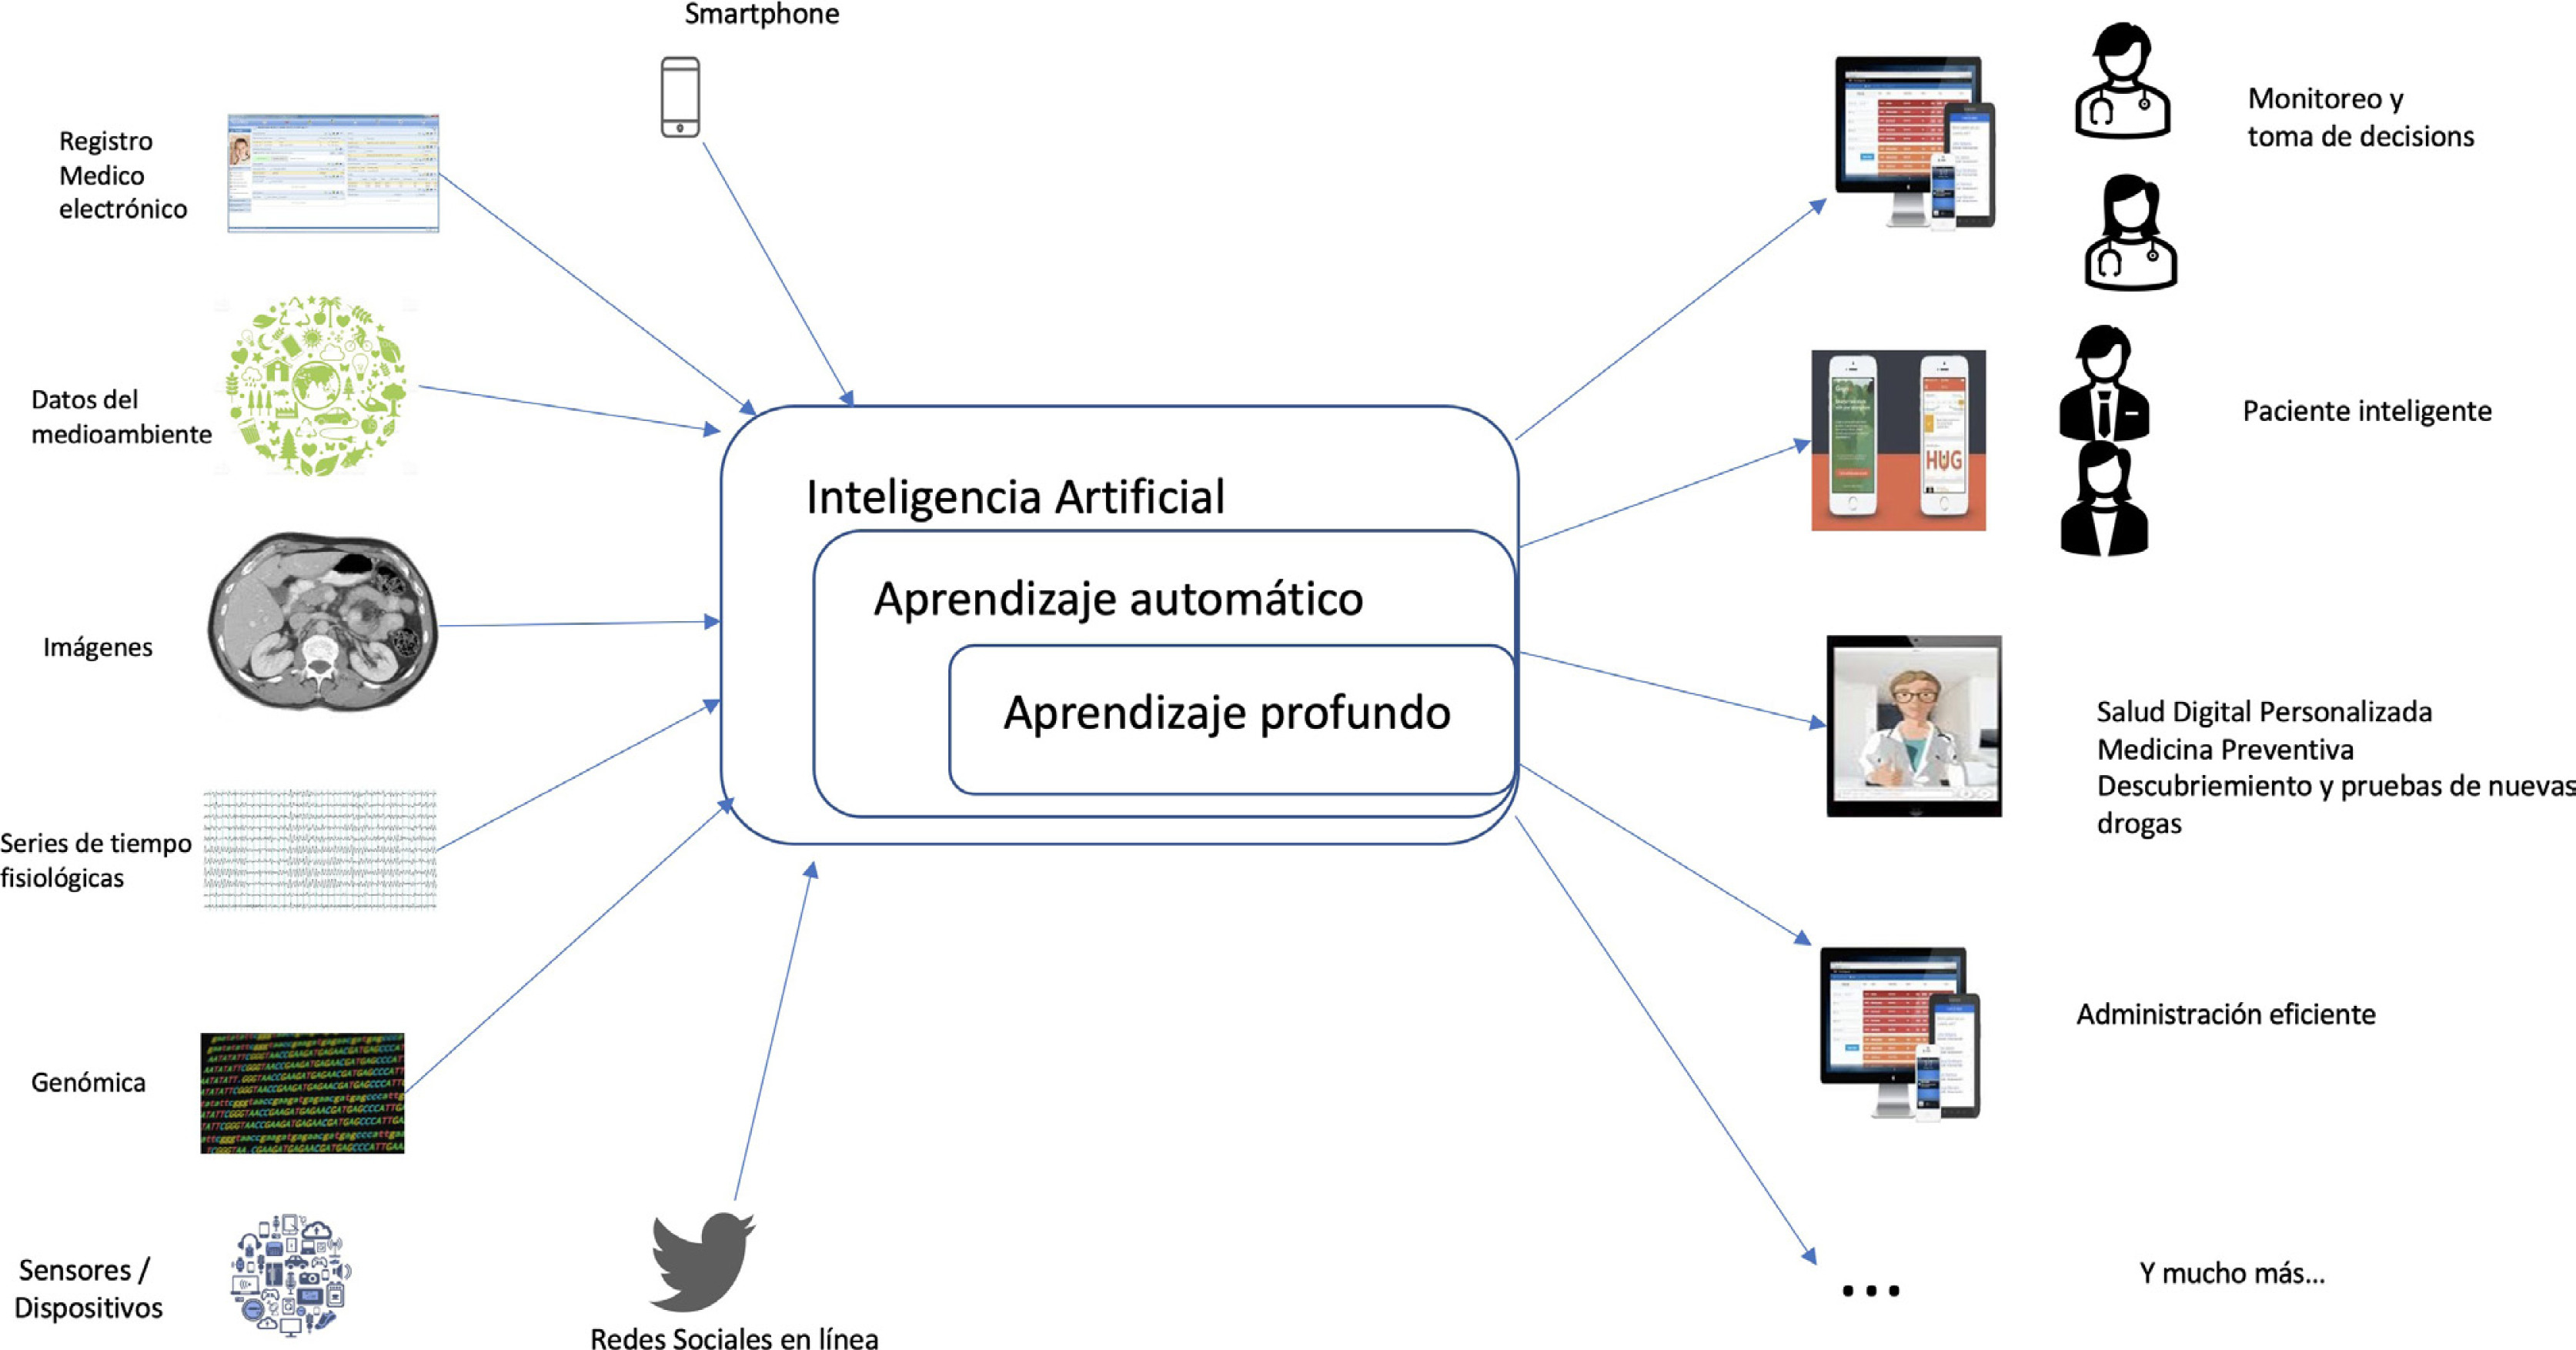
\includegraphics[width=1\linewidth]{high_res.jpg}
    \caption{Integración de varias fuentes de datos relacionadas con los pacientes y el procesamiento respectivo, mediante técnicas de inteligencia artificial.}
    \label{fig:enter-label}
\end{figure}


    \subsection{Inteligencia Artificial en las diferentes áreas de aplicación sanitaria}
        
        
        La IA ha comenzado a incorporarse a la medicina para mejorar la atención al paciente al acelerar los procesos y lograr una mayor precisión diagnóstica, abriendo el camino para brindar una mejor atención médica en general. Las imágenes radiológicas, las preparaciones de anatomía patológica y los registros médicos electrónicos de los pacientes se están evaluando mediante aprendizaje automático ayudando en el proceso de diagnóstico y tratamiento de los pacientes.

        
        De esta manera existen proyectos en la actualidad dedicados a explorar las aplicaciones de la IA en todas las facetas sanitarias: asistencial (prevención de enfermedades, diagnóstico, tratamiento y seguimiento de pacientes), docente o formación continuada, investigadora y gestora. A continuación, se comentan algunos ejemplos concretos en las diferentes áreas de aplicación sanitaria.
\begin{enumerate}
    \item Asistencial: Prevención de enfermedades y diagnóstico precoz: Existen algoritmos informáticos que son capaces de contribuir a la prevención del cáncer de cérvix con alta precisión, ya sea a través de aplicación de software de machine learning en la identificación del virus del papiloma humano o de células con transformaciones oncogénicas. Otros numerosos estudios se están realizando para ofrecer un diagnóstico precoz a través del uso de este tipo de algoritmos en el cáncer de útero, cabeza y cuello, próstata o piel, ya sea a través de la aplicación de este tipo de software a la identificación de proteínas, a técnicas de imagen o a imágenes fotográficas identificando patrones de repetición. También se han desarrollado programas para la detección precoz de cardiopatías ocultas a partir de registros electrocardiográficos digitalizados, diabetes mellitus y sistemas inteligentes que siguen el paradigma del Razonamiento Basado en Casos (Case-Based Reasoning [CBR]) para solucionar problemas actuales mediante la información que tenemos de problemas similares ocurridos anteriormente como el sistema InNoCBR, para la detección y clasificación de casos de infección nosocomial, implantado desde 2013 en el Complexo Hospitalario Universitario de Ourense (CHUO) y desde 2018 extendido a más centros de la comunidad autónoma. Sobre el contenido de mensajes publicados en redes sociales también se pueden generar algoritmos que predicen el riesgo de psicopatologías. Se están desarrollando estudios sobre contenido de publicaciones y su relación con procesos psicológicos como el riesgo de depresión según los contenidos de las redes sociales como Twitter® o Instagram®. A través de la interpretación de datos que registran nuestros movimientos (a través de sensores en nuestro teléfono móvil, reloj inteligente u otros dispositivos) se pueden identificar patrones que sugieran progresión de la enfermedad de Parkinson.
    \item Diagnóstico: Existen muchos programas informáticos de apoyo y ayuda al diagnóstico que han ido mejorando su aprendizaje a través de su uso repetido y continuado. Actualmente existen diferentes tipos de software que se pueden aplicar a diferentes grupos de enfermedades como MYCIN/MYCIN II para enfermedades infecciosas, CASNET para oftalmología, PIP para enfermedades renales o Al/RHEUM para enfermedades reumatológicas. La empresa FDNA a través de su software de reconocimiento facial Face2Gene® es capaz de apoyar o sospechar el diagnóstico de más de 8.000 enfermedades raras, con un reciente ensayo clínico desarrollado en Japón con buenos resultados. En el campo del procesamiento y la interpretación de imágenes para el diagnóstico, la IA ofrece algoritmos que mejoran la calidad y la precisión del diagnóstico ya que los métodos de IA son excelentes para reconocer automáticamente patrones complejos en los datos de imágenes, elimina ruido en las imágenes ofreciendo una mayor calidad y permite establecer modelos tridimensionales a partir de imágenes de pacientes concretos. Investigadores de IBM publicaron una investigación en torno a un nuevo modelo de IA que puede predecir el desarrollo del cáncer de mama maligno, con tasas comparables a las de los radiólogos humanos. Este algoritmo aprende y toma decisiones tanto de datos de imágenes como del historial de la paciente, pudo predecir correctamente el desarrollo del cáncer de mama en el 87\% de los casos analizados, y también pudo interpretar el 77\% de los casos no cancerosos. Este modelo podría algún día ayudar a los radiólogos a confirmar o negar casos positivos de cáncer de mama. Si bien los falsos positivos pueden causar una enorme cantidad de estrés y ansiedad indebidos, los falsos negativos a menudo pueden obstaculizar la detección temprana y el tratamiento posterior de un cáncer. Cuando se puso a prueba frente a 71 casos diferentes que los radiólogos habían determinado originalmente como «no malignos», pero que finalmente terminaron siendo diagnosticados con cáncer de mama dentro del año, el sistema de IA pudo identificar correctamente el cáncer de mama en el 48\% de las personas (48\% de los 71 casos), que de lo contrario no se habrían detectado.
    \item Tratamiento: Combinando diferentes aplicaciones tecnológicas como localización GPS, IA, sensores corporales en tejidos inteligentes o complementos de vestido podemos predecir comportamientos o actividades de personas mayores que viven solas pudiendo mejorar su autonomía. No obstante, existen importantes consideraciones éticas a este respecto por el conflicto existente entre la tranquilidad de los familiares y los cuidadores, y la autonomía, privacidad, dignidad y consentimiento de los ancianos. La IA también se puede aplicar para predecir reacciones adversas de tratamientos médicos o el grado de cumplimentación del tratamiento por parte de los pacientes. Se ha utilizado el procesamiento de lenguaje natural para identificar palabras y frases en informes clínicos que predijeron la fuga anastomótica después de resecciones colorrectales. Muchas de sus predicciones reflejaban el conocimiento clínico que tendría un cirujano, pero este algoritmo también fue capaz de ajustar frases que describen a los pacientes (por ejemplo, irritado, cansado) en el primer día del postoperatorio para lograr predicciones con una sensibilidad del 100\% y una especificidad del 72\%. El uso de los robots quirúrgicos, es una realidad cotidiana en nuestro medio, sobre todo en cirugía prostática, colorrectal o pancreática al considerarse un método menos invasivo. Además de los desarrollos comerciales existentes, se están desarrollando sistemas de asistencia robótica en cirugía de código abierto como el sistema Raven II que será probado en diferentes universidades estadounidenses.
    \item Seguimiento, soporte y monitorización: Muchos asistentes robóticos dotados de sistemas de IA con aplicaciones en salud están desarrollándose en la actualidad fundamentalmente en funciones de información, comunicación y acompañamiento de personas. Normalmente están dotados de un sistema de cámara (permiten moverse en el espacio e incluso detectar emociones a través del reconocimiento facial), sistemas de movilidad, sistemas de escucha e interpretación de voz y otras funciones mecánicas. Pillo es un robot alejado de formas humanoides que una vez programado es capaz de reconocer nuestra voz, nuestra cara y ofrecernos la medicación a la hora correcta. Las medicinas se cargan en un compartimento específico donde se mantienen en perfecto estado de conservación, es capaz de reconocer la medicación prescrita a cada miembro de la familia y responder a sencillas preguntas sobre alimentación y ejercicio. Almacena algunas variables de salud sobre cada uno de los miembros de la familia (peso, talla, niveles de glucemia y colesterol, tensión arterial...). Además de reconocer a cada una de las personas y poder ofrecerles la medicación correspondiente sin equivocarse abre caminos de futuro:
    
\begin{itemize}
    \item Una vez que se haya adelantado en el reconocimiento facial e interpretación de gestos podría establecer comunicación con dispositivos de asistencia domiciliaria urgente y videoconferencias ante situaciones de alerta de salud de la persona a quien cuida.
    \item Podría ser un sistema de comunicación automática con dispositivos sociosanitarios.
    \item Podría ser un entrenador en habilidades y ejercicios de rehabilitación física o mental.
\end{itemize}
    
\end{enumerate}

    \subsection{Inteligencia Artificial en las diferentes especialidades médicas}
    
    La evolución de numerosas áreas médicas con el uso de la IA ha sido impresionante: por ejemplo, la radiología, que en las últimas décadas ha sido líder en la transformación digital de imágenes, sistemas de archivo y comunicación de imágenes (PACS), y la telerradiología, pues con el uso de IA ha dado lugar a la aparición de nuevas áreas como la radiómica, que con el uso de algoritmos y software integra y correlaciona datos de radiología, patología y genómica. Se espera que, con la ayuda de la IA, la interpretación de imágenes sea mejor y más rápida. Un algoritmo será capaz de alimentarse de muchas imágenes y partes de datos que le permitan aprender y detectar diferencias en los tejidos, y apoyar al médico radiólogo con informes diagnósticos asistidos por computadora que agilizarán su actividad diaria. La IA no reemplazará a los radiólogos, pero los radiólogos que usen IA reemplazarán a los que no lo hagan.
    
    
    En la actualidad, los sistemas de salud se enfrentan a una escasez global de patólogos, mientras que la carga de trabajo y la complejidad diagnóstica siguen aumentando. La incorporación de la patología digital y la implementación de diagnósticos asistidos por algoritmos de IA transformarán la práctica de la patología, mejorando el tiempo de entrega de los resultados, la eficiencia y la precisión diagnóstica de los médicos patólogos. En un metaanálisis de 24 estudios se observó una concordancia general del 98.3\% entre la patología digital con microscopía virtual (Whole Slide Imaging [WSI]) y con microscopía de luz para el diagnóstico de rutina. Hoy es posible dicotomizar automáticamente, mediante algoritmos de IA, lesiones benignas y malignas de mama con un área bajo la curva de 0.962 y una precisión del 81.3\% para diferenciar lesiones benignas de carcinomas ductales in situ e invasivos de mama.
    
    
    En cardiología, el uso de la IA se ha estudiado en la predicción de hipertensión esencial, la detección de fibrilación auricular por relojes inteligentes, la clasificación de estenosis aórtica por análisis de señales cardiomecánicas en sensores inalámbricos portátiles, la clasificación de arritmias mediante electrocardiograma de una sola derivación, etc.
    
    
    En neurología se han estudiado la predicción de la recurrencia de eventos vasculares cerebrales isquémicos, la evaluación prequirúrgica de la epilepsia resistente a fármacos, la predicción de la enfermedad de Alzheimer y el diagnóstico de la enfermedad de Parkinson.
   
    
    En oftalmología, en el año 2018, la Food and Drug Administration aprobó el primer software de IA para el diagnóstico de retinopatía diabética en consultorios de atención primaria, y ha logrado un rendimiento diagnóstico extraordinario en la detección de glaucoma, arco corneal, cataratas, degeneración macular y retinopatía del prematuro.
    
    
    En dermatología, la IA está mejorando la eficiencia y la precisión de los enfoques diagnósticos tradicionales, incluidos el examen visual, la biopsia de piel y el estudio histopatológico. Numerosos estudios han reportado la precisión diagnóstica de la IA, igual o mejor que la de los dermatólogos, en lesiones cutáneas a partir de imágenes clínicas y dermatoscópicas. Su utilidad inicial consistió en la detección del melanoma y de lesiones cutáneas pigmentarias, pero en la actualidad incluye la detección de enfermedades como la queratosis seborreica y la psoriasis. Las aplicaciones de la IA en dermatología incluyen asimismo áreas de diagnóstico, como la teledermatología (triaje de lesiones cutáneas), y de dermatopatología, pero también serán de utilidad en el pronóstico y el tratamiento de las enfermedades de la piel.
    
    
    Las oportunidades de la IA en el ámbito quirúrgico incluyen herramientas útiles en el periodo preoperatorio, con la toma de decisiones quirúrgicas, la identificación de factores de riesgo modificables y el procesamiento de imágenes que mejoran la planeación quirúrgica de procedimientos percutáneos (p. ej., ablación tumoral), estereotácticos (p. ej., neuroquirúrgicos), ortopédicos (p. ej., elección de tamaño adecuado de una prótesis), cardiovasculares (p. ej., elección de una prótesis valvular) y laparoscópicos (p. ej., mejor sitio de incisión y colocación de instrumentos quirúrgicos).
    \\Durante el evento quirúrgico, los cirujanos deben tomar decisiones complejas y de alto riesgo bajo limitaciones de tiempo, que con frecuencia tienen un efecto significativo en el pronóstico de los pacientes. Una nueva disciplina de la IA, denominada ciencia de datos quirúrgicos, registra y analiza variables intraoperatorias (p. ej., signos vitales, estudios de imagen, etc.) que ayudan al cirujano a tomar decisiones compartidas de tratamiento. En el posoperatorio, la IA puede ayudar en la detección temprana y el tratamiento de complicaciones, y en un futuro, los sistemas quirúrgicos robóticos teleoperados permitirán al cirujano brindar atención en ubicaciones remotas.
   
    
    En psiquiatría, el uso de IA será particularmente útil en el diagnóstico y el tratamiento de enfermedades psiquiátricas; se planea que en el futuro será posible analizar el estado emocional de los pacientes con dispositivos portátiles que analicen la voz, el comportamiento, el sueño, el apetito, etc. El médico psiquiatra podrá apoyarse en la elección del psicofármaco basado en datos de neuroimagen, farmacogenéticos y clínicos del paciente, ofreciendo una terapia específica y practicando medicina de precisión. \cite{lanzagorta-ortega_inteligencia_2023}

    
\vspace{0.5cm}
        \begin{tabularx}{0.8\textwidth} { |m{2.3cm}| m{9.7cm} |}
        \hline
        \textbf{Área sanitaria} &\textbf{Aplicación} 
        \\
        \hline
        {Asistencial} & {Prevención de enfermedades y diagnóstico precoz: Algoritmos para prevenir cáncer de cérvix, identificación de virus del papiloma humano, diagnóstico precoz de cáncer de útero, cabeza, cuello, próstata y piel.} \\ 
        \hline                            
        {Diagnóstico} & {Software de apoyo al diagnóstico, como Face2Gene para enfermedades raras, algoritmos de interpretación de imágenes para mejorar la precisión diagnóstica, incluyendo cáncer de mama.} \\ 
        \hline
        {Tratamiento} & {Aplicación de IA en combinación con tecnologías como GPS, sensores corporales, para predecir comportamientos de personas mayores y prever reacciones adversas a tratamientos médicos.} \\ 
        \hline
        {Seguimiento y monitorización} & {Asistentes robóticos con IA para información, comunicación y acompañamiento, como el robot Pillo.}  \\
        \hline
        \end{tabularx} 
        
        \caption{Tabla 1: Resumen de la aplicación de IA en las diferentes áreas sanitarias}
        \label{tab:1}
        
\vspace{0.5cm}
\begin{center}
    \section{Implicaciones éticas del empleo de la Inteligencia Artificial en la Medicina}
\end{center}


La automatización y   la   inclusión   de   los   robots y las máquinas en general en la toma de decisiones que afectan a los seres humanos conllevan una serie de consideraciones éticas de   gran   importancia.   Por un lado, la capacidad de cálculo por parte de las máquinas es mucho más rápida y precisa que la humana, pero existen variables no numéricas relacionadas con aspectos no tangibles que las máquinas aún no son capaces de incluirlas en sus procesos de decisión.


Tener robots que realizan tareas mecánicas en situaciones de gran riesgo para los seres humanos (entornos contaminados biológicamente o de gran toxicidad, desactivación de explosivos, reparaciones en entornos incompatibles con la vida humana como grandes profundidades o medición de variables en situaciones extremas como el viento en un huracán) suponen una ventaja considerable para la sociedad.


Los robots que realizan actividades cotidianas y repetitivas (realización de cientos de tests analíticos de laboratorio) suponen una descarga de tareas para el ser humano, pero esto puede provocar la desaparición de puestos de trabajo.


Disponer de robots que realizan tareas complejas para la toma de decisiones (por ejemplo, diagnósticos) tiene unas implicaciones éticas de gran importancia. La Unión Europea ha elaborado una guía de consideraciones éticas en la que se proponen tres principios básicos para conseguir una IA fiable:
        \begin{enumerate}
            \item Asegurarse de que la IA esté centrada en el ser humano: La IA se debe desarrollar, implementar y utilizar con un «propósito ético», fundamentado y que refleje los derechos fundamentales, los valores sociales y los principios éticos de la Beneficencia (hacer el bien), Maleficencia (no hacer daño), Autonomía de los seres humanos, Justicia y Explicabilidad.
            \item Confiar en los derechos fundamentales, principios éticos y valores para evaluar prospectivamente los posibles efectos de la IA en los seres humanos y el bien común. Prestar especial atención a las situaciones que involucran a los grupos más vulnerables, como niños, personas con discapacidades o minorías, o situaciones con asimetrías de poder o información, como entre empleadores y empleados, o empresas y consumidores.
            \item Reconocer y tener en cuenta el hecho de que, si bien aporta beneficios sustanciales a los individuos y a la sociedad, la IA también puede tener un impacto negativo. Permanecer atento a las áreas de preocupación crítica. Para asegurar estos principios se han elaborado una serie de recomendaciones (tabla 2).
        \end{enumerate}
Además de la gran importancia de tener una normativa ética en la creación, desarrollo, implementación y evaluación de sistemas de IA hay otro proceso clave en este sentido.


La mayoría de sistemas de IA se basan en técnicas de aprendizaje automático a través de grandes colecciones de datos. Por lo tanto, una posible manera de generar sesgos en la toma de decisiones de la IA puede tener en la recopilación y selección de datos de entrenamiento. Si los datos de capacitación no son lo suficientemente inclusivos y equilibrados, el sistema podría aprender a tomar decisiones injustas, por ejemplo, los sistemas de reconocimiento facial son más fiables en varones blancos que en mujeres negras hecho que se está corrigiendo gracias al Gender Shades Projetc.


La clave no es si existe algún sesgo; sino si el sesgo creado por los datos, las preguntas y las prioridades o los valores es moralmente neutro. Si es así, entonces el resultado será equitativo. \cite{avila-tomas_inteligencia_2021}
        
\vspace{0.5cm}
        \begin{tabularx}{0.8\textwidth} { |p{1cm}| m{11cm} |}
        \hline
        {1} &{Incorporar los requisitos para la IA de confianza desde la primera fase de diseño.} 
        \\
        \hline
        {2} & {Considerar métodos técnicos y no técnicos para garantizar la implementación de esos requisitos en el sistema de IA. Además, tener en cuenta esos requisitos para construir el equipo, para trabajar en el sistema en sí, el entorno de prueba y las aplicaciones potenciales del sistema.} \\ 
        \hline                            
        {3} & {Proporcionar de manera clara y proactiva información a las partes interesadas (clientes, empleados, etc.) sobre     las capacidades y limitaciones del sistema de IA, lo que nos permite establecer expectativas realistas. Asegurar la trazabilidad del sistema de IA es clave en este sentido.} \\ 
        \hline
        {4} & {Hacer que la IA confiable sea parte de la cultura de la organización, y brindar información a las partes interesadas sobre la implementación, el diseño y el uso de los sistemas de IA. La IA confiable también se puede incluir en deontología o códigos de conducta de las organizaciones.} \\ 
        \hline
        {5} & {Asegurar la participación e inclusión de las partes interesadas en el diseño y desarrollo del sistema de IA. Además, asegure la diversidad al configurar los equipos que desarrollan, implementan y prueban el producto.}  \\
        \hline
        {6} & {Prever formación y educación y asegurarse de que los directivos, desarrolladores, usuarios y empleadores conozcan y estén capacitados en IA confiable.}  \\
        \hline
        {7} & {Esforzarse por facilitar la auditabilidad de sistemas de IA, particularmente en contextos o situaciones críticas.}  \\
        \hline
        {8} & {Considerar la posible existencia de conflictos entre             diferentes objetivos (la transparencia puede abrir la puerta al mal uso; identificar y corregir sesgos puede   contrastar con las protecciones de privacidad). Comunicar y documentar estas compensaciones.}  \\
        \hline
        {9} & {Fomentar la investigación y la innovación para promover el cumplimiento de los requisitos para la IA   confiable.}  \\
        \hline
        \end{tabularx} 
        \\
        \caption {\\Tabla 2 : Recomendaciones del High-Level Expert Group on Artificial Intelligence. Draft Ethics Guidelines for Trust- worthy AI. European Commission}
        \label{tab:2}

        
En EE. UU. el Instituto Future of Life ha desarrollado los Principios de Inteligencia Artificial en Asilomar (Monterrey, California) a través de una conferencia con un amplio panel de expertos en robótica, físicos, economistas, filósofos y otros expertos en sus áreas en enero de 2017 donde se ha generado un consenso en varias recomendaciones.
        
        \subsubsection{Principios de la IA de Asilomar}
        
        \begin{itemize}
                    
            \item Objetivo de investigación: sus objetivos deben ser crear inteligencia no dirigida, pero beneficiosa.
            \item Financiación de la investigación: las inversiones en IA deben ir acompan˜adas de financiación para la investigación sobre cómo garantizar su uso beneficioso, incluidas preguntas espinosas en informática, economía, derecho, ética y estudios sociales.
            \item Enlace ciencia-política: debe haber una relación constructiva y saludable entre los investigadores de IA y los responsables políticos.
            \item Cultura de la investigación: debe fomentarse una cultura de cooperación, confianza y transparencia entre los investigadores y desarrolladores de IA.
            \item Evitar las carreras: los equipos que desarrollan sistemas de inteligencia artificial deben cooperar activamente para evitar el recorte de las normas de seguridad.
            \item Seguridad: los sistemas de IA deben ser seguros de manera verificable durante toda su vida operativa.
            \item Transparencia de fallos: si un sistema de IA causa daño, debería ser posible determinar la causa.
            \item Transparencia judicial: cualquier participación de un sistema autónomo en la toma de decisiones judiciales debe proporcionar una explicación satisfactoria auditable por una autoridad humana competente.
            \item Alineación del valor de los sistemas de IA con los valores humanos a lo largo de su operación.
            \item Valores humanos: los sistemas de IA deben disen˜arse y operarse de manera que sean compatibles con los ideales de dignidad humana, derechos, libertades y diversidad cultural.
            \item Privacidad personal: las personas deben tener derecho de acceso, administración y control de los datos que generan, debido al poder de los sistemas de IA para analizar y utilizar esos datos. 
            \item Libertad y privacidad: la aplicación de la IA a los datos personales no debe limitar injustificadamente la libertad real o percibida de las personas.
            \item Beneficio compartido: las tecnologías de IA deberían beneficiar y capacitar a tantas personas como sea posible.
            \item Prosperidad compartida: la prosperidad económica creada por una IA debe compartirse ampliamente en beneficio de toda la humanidad.
            \item Control humano: los seres humanos deben elegir cómo, y si delegar decisiones a los sistemas de IA para lograr los objetivos elegidos por el hombre. 
            \item No subversión: el poder conferido por el control de sistemas de IA altamente avanzados debe respetar y mejorar, en lugar de subvertir, los procesos sociales y cívicos de los que depende la salud de la sociedad.
            \item Carrera armamentista de la IA: se debe evitar una carrera armamentista en armas autónomas letales.
            \item Precaución sobre la capacidad: al no haber consenso, debemos evitar suposiciones sólidas con respecto a los límites superiores de las capacidades futuras de IA.
            \item Importancia: la IA avanzada podría representar un cambio profundo en la historia de la vida en la tierra, y debería planearse y manejarse con cuidados y recursos proporcionales.
            \item Riesgos: los riesgos que plantean los sistemas de IA, especialmente los riesgos catastróficos o existenciales, deben estar sujetos a los esfuerzos de planificación y mitigación acordes con el impacto esperado.
            \item Auto-mejora recursiva: los sistemas de IA disen˜ados para auto-replicarse o auto-replicarse de manera recursiva de una manera que podría llevar a un aumento rápido de la calidad o cantidad deben estar sujetos a estrictas medidas de seguridad y de control.
            \item Bien común: la superinteligencia solo debe desarrollarse al servicio de ideales éticos ampliamente compartidos, y en beneficio de toda la humanidad en lugar de un estado u organización.\cite{avila-tomas_inteligencia_2021}

        \end{itemize}

        
    
\begin{center}
    \section{Conclusiones}
\end{center}

        \begin{itemize}
            \item La IA ha experimentado un crecimiento significativo en la investigación aplicada a la Medicina en la última década, mejorando la eficiencia y eficacia de la prestación de servicios de salud.
            \item La capacidad de los algoritmos de IA para analizar grandes cantidades de datos ha revolucionado la prevención, diagnóstico y tratamiento de diversas enfermedades, contribuyendo a la identificación temprana y personalizada de condiciones médicas.
            \item A pesar de los avances positivos, el uso de la IA en Medicina plantea desafíos éticos, especialmente en la gestión de datos médicos sensibles, que requieren medidas de seguridad y consideraciones éticas rigurosas.
            \item La Unión Europea ha establecido principios para guiar el desarrollo ético de la IA en Medicina, enfocándose en centrar la IA en el ser humano, garantizar valores éticos y abogar por la privacidad y la equidad.
        \end{itemize}

\vspace{0.5cm}

\nocite{*}
\begin{center}
   \printbibliography[title={Referencias}]
\end{center}

    
\end{document}